\section{Actividad 2.1: Conversor de BCD a Exceso-3}

Diseñar y armar un conversor de código BCD a XS3 (exceso 3).
Realizar:
\begin{itemize}
    \item Tabla de verdad.
    \item Obtener las funciones lógicas de salidas con circuitos combinacionales.
    \item Minimizar las funciones canónicas obtenidas de la tabla de verdad.
    \item Armar el circuito y verificar su funcionamiento en el MiniLab.
    \item Armar el circuito y verificar su funcionamiento en el simulador “falstad.com”
\end{itemize}


\subsection{Tabla de verdad}

\begin{center}
\centering
\begin{tabular}{c c c c || c c c c}
A & B & C & D & W & X & Y & Z \\
\hline
0 & 0 & 0 & 0 & 0 & 0 & 1 & 1 \\
0 & 0 & 0 & 1 & 0 & 1 & 0 & 0 \\
0 & 0 & 1 & 0 & 0 & 1 & 0 & 1 \\
0 & 0 & 1 & 1 & 0 & 1 & 1 & 0 \\
0 & 1 & 0 & 0 & 0 & 1 & 1 & 1 \\
0 & 1 & 0 & 1 & 1 & 0 & 0 & 0 \\
0 & 1 & 1 & 0 & 1 & 0 & 0 & 1 \\
0 & 1 & 1 & 1 & 1 & 0 & 1 & 0 \\
1 & 0 & 0 & 0 & 1 & 0 & 1 & 1 \\
1 & 0 & 0 & 1 & 1 & 1 & 0 & 0 \\
1 & 0 & 1 & 0 & x & x & x & x \\
1 & 0 & 1 & 1 & x & x & x & x \\
1 & 1 & 0 & 0 & x & x & x & x \\
1 & 1 & 0 & 1 & x & x & x & x \\
1 & 1 & 1 & 0 & x & x & x & x \\
1 & 1 & 1 & 1 & x & x & x & x \\
\end{tabular}
\\Tabla de verdad para el conversor BCD a Exceso-3
\end{center}

\subsection{Funciones lógicas de salida}
\begin{itemize}
    \item $W = \overline{A} \cdot B \cdot \overline{C} \cdot D + \overline{A} \cdot B \cdot C \cdot \overline{D} + \overline{A} \cdot B \cdot C \cdot D + A \cdot \overline{B} \cdot \overline{C} \cdot \overline{D} + A \cdot \overline{B} \cdot \overline{C} \cdot D$
    \item $X = \overline{A} \cdot \overline{B} \cdot \overline{C} \cdot D + \overline{A} \cdot \overline{B} \cdot C \cdot \overline{D} + \overline{A} \cdot \overline{B} \cdot C \cdot D  + \overline{A} \cdot B \cdot \overline{C} \cdot \overline{D} + A \cdot \overline{B} \cdot \overline{C} \cdot D$
    \item $Y = \overline{A} \cdot \overline{B} \cdot \overline{C} \cdot \overline{D} + \overline{A} \cdot \overline{B} \cdot C \cdot D + \overline{A} \cdot B \cdot \overline{C} \cdot \overline{D} + \overline{A} \cdot B \cdot C \cdot D + A \cdot \overline{B} \cdot \overline{C} \cdot \overline{D}$
    \item $Z = \overline{A} \cdot \overline{B} \cdot \overline{C} \cdot \overline{D} + \overline{A} \cdot \overline{B} \cdot C \cdot \overline{D} + \overline{A} \cdot B \cdot \overline{C} \cdot \overline{D} + \overline{A} \cdot B \cdot C \cdot \overline{D} + A \cdot \overline{B} \cdot \overline{C} \cdot \overline{D}$
\end{itemize}

\subsection{Minimización por mapas de Karnaugh}

\begin{center}
\centering
\renewcommand{\arraystretch}{1.5}
\begin{tabular}{c|cccc}
\diagbox{AB}{CD} & 00 & 01 & 11 & 10 \\
\hline
00 & 0 & 0 & 0 & 0 \\
01 & 0 & 1 & 1 & 1 \\
11 & x & x & x & x \\
10 & 1 & 1 & x & x \\
\end{tabular}
Salida W
\end{center}
\begin{itemize}
    \item $W = B\cdot D + B \cdot C + A$
\end{itemize}

\begin{center}
\centering
\renewcommand{\arraystretch}{1.5}
\begin{tabular}{c|cccc}
\diagbox{AB}{CD} & 00 & 01 & 11 & 10 \\
\hline
00 & 0 & 1 & 1 & 1 \\
01 & 1 & 0 & 0 & 0 \\
11 & x & x & x & x \\
10 & 0 & 1 & x & x \\
\end{tabular}
Salida X
\end{center}
\begin{itemize}
    \item $X = B \cdot \overline{C} \cdot \overline{D} + \overline{B} \cdot D + \overline{B} \cdot C$
\end{itemize}

\begin{center}
\centering
\renewcommand{\arraystretch}{1.5}
\begin{tabular}{c|cccc}
\diagbox{AB}{CD} & 00 & 01 & 11 & 10 \\
\hline
00 & 1 & 0 & 1 & 0 \\
01 & 1 & 0 & 1 & 0 \\
11 & x & x & x & x \\
10 & 1 & 0 & x & x \\
\end{tabular}
Salida Y
\end{center}
\begin{itemize}
    \item $Y = \overline{C} \cdot \overline{D} + C \cdot D$
\end{itemize}

\begin{center}
\centering
\renewcommand{\arraystretch}{1.5}
\begin{tabular}{c|cccc}
\diagbox{AB}{CD} & 00 & 01 & 11 & 10 \\
\hline
00 & 1 & 0 & 0 & 1 \\
01 & 1 & 0 & 0 & 1 \\
11 & x & x & x & x \\
10 & 1 & 0 & x & x \\
\end{tabular}
Salida Z
\end{center}
\begin{itemize}
    \item $W = \overline{D} $
\end{itemize}

\saltoPag

\subsection{Circuito lógico en Falstad}

\begin{figure}[h!]
    \centering
    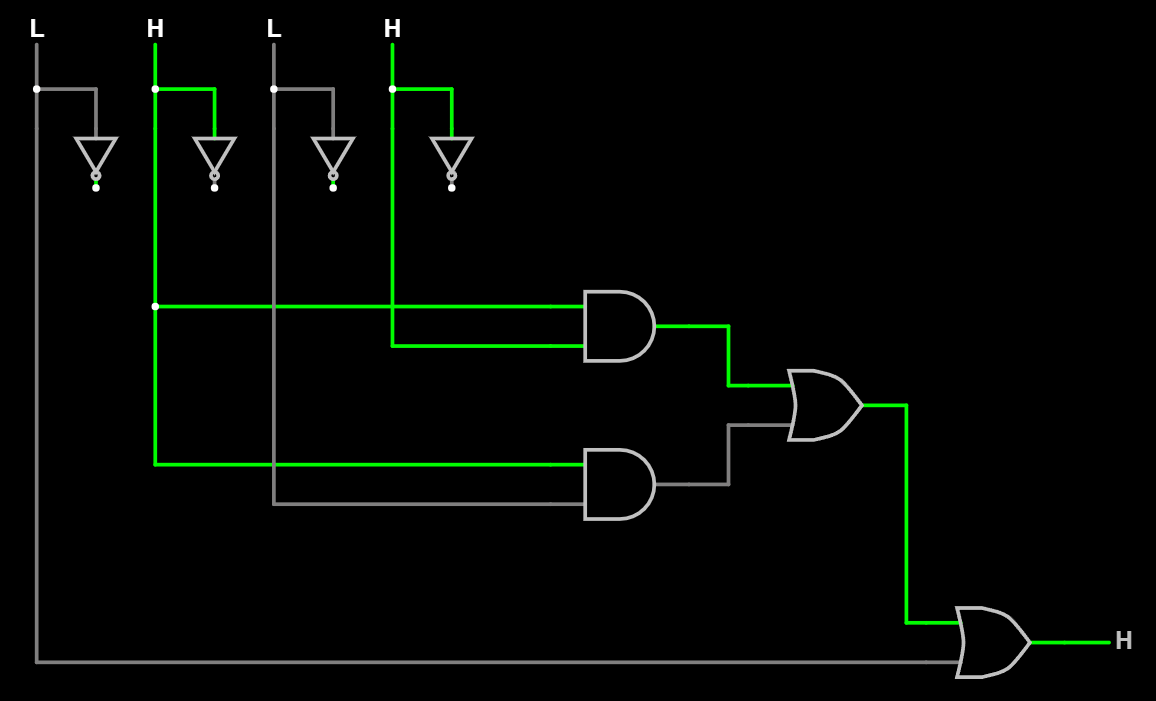
\includegraphics[width=7cm]{imagenes/2.1_W.png}
    \caption{Circuito lógico implementado en Falstad para $W$}
    \label{fig:falstad}
    \footnotesize\textit{Bits usados para ejemplo 0101.}
\end{figure}

\begin{figure}[h!]
    \centering
    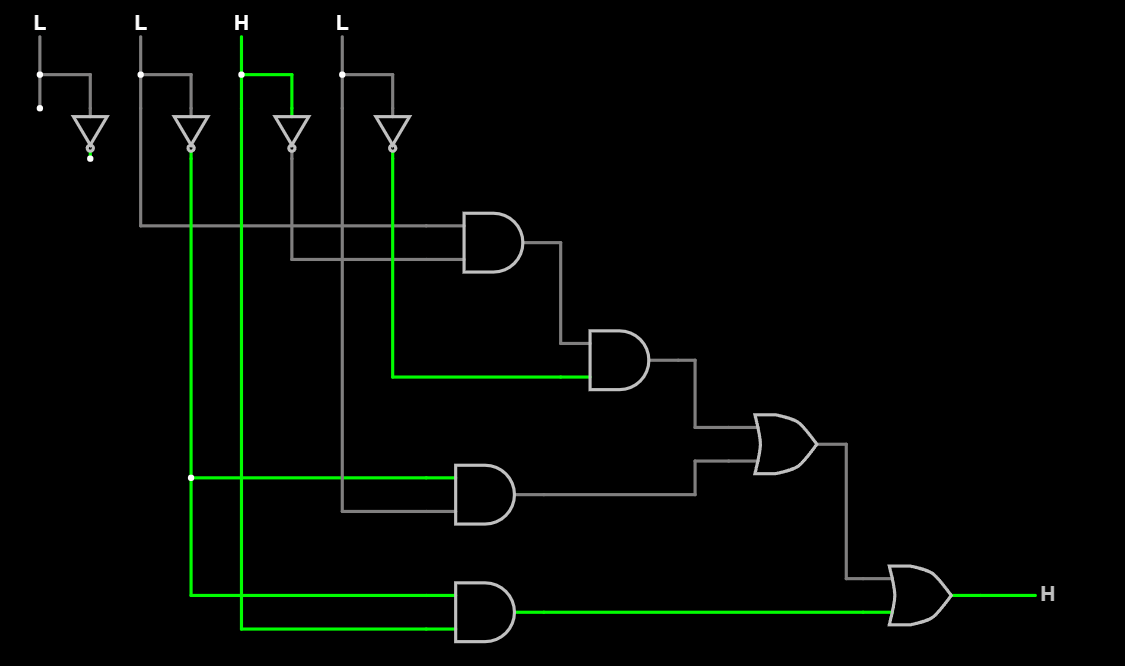
\includegraphics[width=7cm]{imagenes/2.1_X.png}
    \caption{Circuito lógico implementado en Falstad para $X$}
    \label{fig:falstad}
    \footnotesize\textit{Bits usados para ejemplo 0010.}
\end{figure}

\begin{figure}[h!]
    \centering
    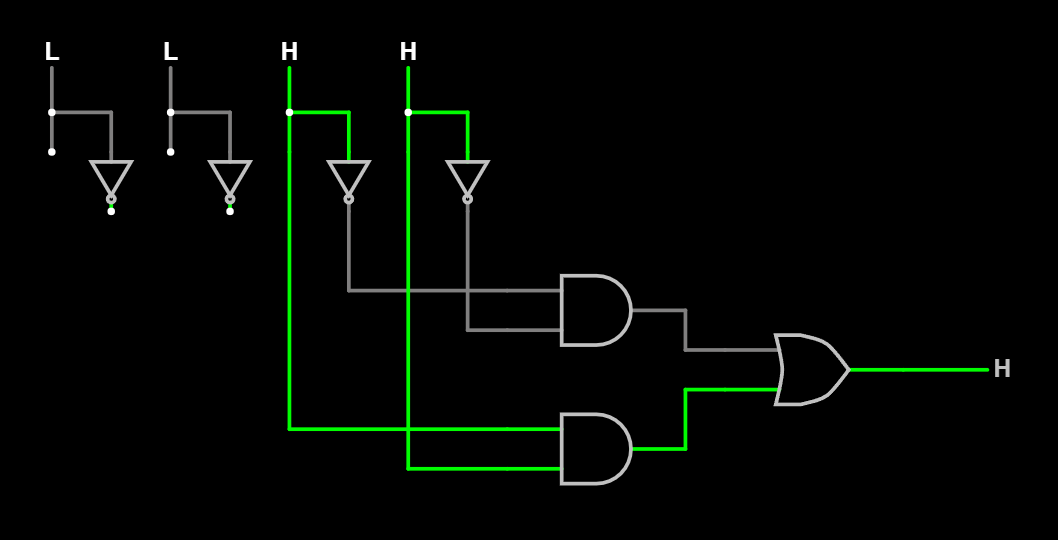
\includegraphics[width=7cm]{imagenes/2.1_Y.png}
    \caption{Circuito lógico implementado en Falstad para $Y$}
    \label{fig:falstad}
    \footnotesize\textit{Bits usados para ejemplo 0011.}
\end{figure}

\begin{figure}[h!]
    \centering
    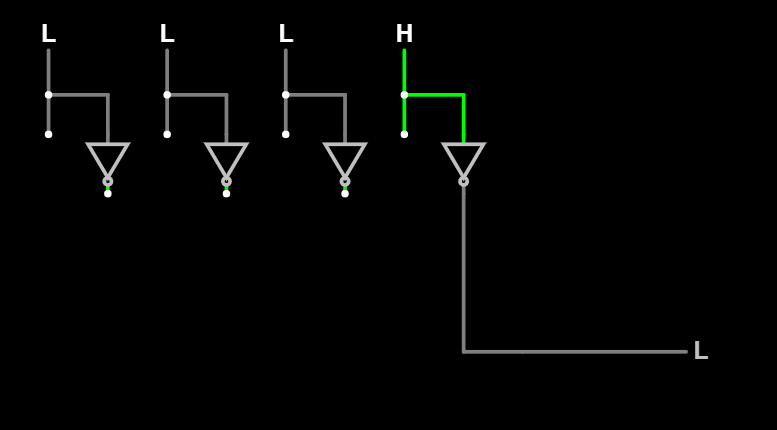
\includegraphics[width=7cm]{imagenes/2.1_Z.png}
    \caption{Circuito lógico implementado en Falstad para $Z$}
    \label{fig:falstad}
    \footnotesize\textit{Bits usados para ejemplo 0001.}
\end{figure}



\saltoPag

\section{Actividad 2.2: Comparador Binario}

El circuito de la figura es un comparador binario de dos números (A y B) de dos bits cada uno. Las
salidas ($S_0$, $S_1$ y $S_2$) representan la salida del comparador y $S0=1$ cuando $A>B$, $S_1= 1$ cuando $A < B$ y
$S_2=1$ $A=B$, en caso de no darse la condición la salida permanece en cero.

% Puedes poner esto en tu archivo actividades.tex donde lo necesites
\begin{figure}[h!]
    \centering
    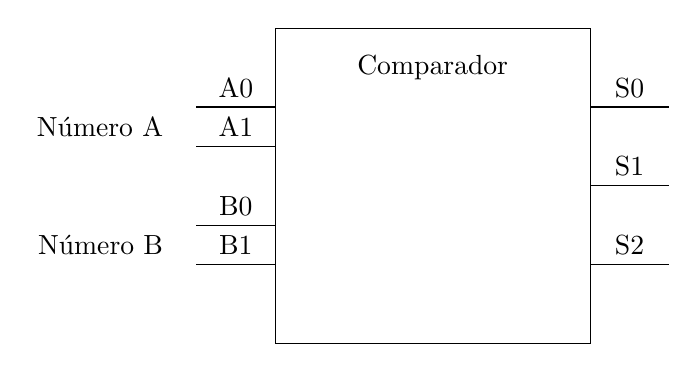
\begin{tikzpicture}[scale=1, every node/.style={scale=1}]
        % Caja del comparador
        \draw (0,0) rectangle (4,4);
        \node at (2,3.5) {Comparador};

        % Entradas A
        \draw[-] (-1,3) -- (0,3);
        \node[above] at (-0.5,3) {A0};
        \draw[-] (-1,2.5) -- (0,2.5);
        \node[above] at (-0.5,2.5) {A1};
        \node[left] at (-1.3,2.75) {Número A};

        % Entradas B
        \draw[-] (-1,1.5) -- (0,1.5);
        \node[above] at (-0.5,1.5) {B0};
        \draw[-] (-1,1) -- (0,1);
        \node[above] at (-0.5,1) {B1};
        \node[left] at (-1.3,1.25) {Número B};

        % Salidas
        \draw[-] (4,3) -- (5,3);
        \node[above] at (4.5,3) {S0};
        \draw[-] (4,2) -- (5,2);
        \node[above] at (4.5,2) {S1};
        \draw[-] (4,1) -- (5,1);
        \node[above] at (4.5,1) {S2};
    \end{tikzpicture}
    \caption{Comparador binario de dos bits}
\end{figure}

Realizar:
\begin{itemize}
 \item Tabla de verdad.
 \item Obtener las funciones lógicas de salidas con circuitos combinacionales.
 \item Minimizar utilizando mapas de Karnaugh.
 \item Minimizar utilizando los teoremas y postulados del algebra de Boole.
 \item Armar el circuito y verificar su funcionamiento en el MiniLab.
 \item Armar el circuito y verificar su funcionamiento en el simulador “falstad.com”
\end{itemize}



\subsection{Tabla de verdad}

\begin{center}
\centering
\begin{tabular}{c c c c || c c c}
A1 & A0 & B1 & B0 & S0 & S1 & S2 \\
\hline
0 & 0 & 0 & 0 & 0 & 0 & 1 \\
0 & 0 & 0 & 1 & 0 & 1 & 0 \\
0 & 0 & 1 & 0 & 0 & 1 & 0 \\
0 & 0 & 1 & 1 & 0 & 1 & 0 \\
0 & 1 & 0 & 0 & 1 & 0 & 0 \\
0 & 1 & 0 & 1 & 0 & 0 & 1 \\
0 & 1 & 1 & 0 & 0 & 1 & 0 \\
0 & 1 & 1 & 1 & 0 & 1 & 0 \\
1 & 0 & 0 & 0 & 1 & 0 & 0 \\
1 & 0 & 0 & 1 & 1 & 0 & 0 \\
1 & 0 & 1 & 0 & 0 & 0 & 1 \\
1 & 0 & 1 & 1 & 0 & 1 & 0 \\
1 & 1 & 0 & 0 & 1 & 0 & 0 \\
1 & 1 & 0 & 1 & 1 & 0 & 0 \\
1 & 1 & 1 & 0 & 1 & 0 & 0 \\
1 & 1 & 1 & 1 & 0 & 0 & 1 \\
\end{tabular}
\\Tabla de verdad del comparador binario de dos bits
\end{center}


\subsection{Funciones lógicas de salida}
\begin{itemize}
    \item $S0 = \overline{A_1} \cdot A_0 \cdot \overline{B_1} \cdot \overline{B_0} + A_1 \cdot \overline{A_0} \cdot \overline{B_1} \cdot \overline{B_1} + A_1 \cdot \overline{A_0} \cdot \overline{B_1} \cdot B_0 + A_1 \cdot A_0 \cdot \overline{B_1} \cdot \overline{B_0} + A_1 \cdot A_0 \cdot \overline{B_1} \cdot B_0 + A_1 \cdot A_0 \cdot B_1 \cdot \overline{B_0}$
    \item $S1 = \overline{A_1} \cdot \overline{A_0} \cdot \overline{B_1} \cdot B_0 + \overline{A_1} \cdot \overline{A_0} \cdot B_1 \cdot \overline{B_0} + \overline{A_1} \cdot \overline{A_0} \cdot B_1 \cdot B_0 + \overline{A_1} \cdot A_0 \cdot B_1 \overline{B_0} + \overline{A_1} \cdot A_0 \cdot B_1 \cdot B_0 + A_1 \cdot \overline{A_0} \cdot B_1 \cdot B_0 $ 
    \item $S2 = \overline{A_1} \cdot \overline{A_0} \cdot \overline{B_1} \cdot \overline{B_0} + \overline{A_1} \cdot A_0 \cdot \overline{B_1} \cdot B_0 + A_1 \cdot \overline{A_0} \cdot B_1 \cdot \overline{B_0} + A_1 \cdot A_0 \cdot B_1 \cdot B_0 $
\end{itemize}


\subsection{Minimización por mapas de Karnaugh}

\begin{center}
\centering
\renewcommand{\arraystretch}{1.5}
\begin{tabular}{c|cccc}
\diagbox{$A_1A_0$}{$B_1B_0$} & 00 & 01 & 11 & 10 \\
\hline
00 & 0 & 0 & 0 & 0 \\
01 & \cellcolor{cyan!30}1 & 0 & 0 & 0 \\
11 & 
    % 1100: tres colores, cada uno ocupa un tercio vertical de la celda
    \tikz{
        \fill[red!30] (0,0) rectangle (0.2,0.5);
        \fill[cyan!30] (0.2,0) rectangle (0.4,0.5);
        \fill[green!30] (0.4,0) rectangle (0.6,0.5);
        \node at (0.3,0.3) {1};
    } &
    \cellcolor{red!30}1 & 0 & \cellcolor{green!30}1 \\
10 & 
    \cellcolor{red!30}1 & 
    \cellcolor{red!30}1 & 
    0 & 
    0 \\
\end{tabular}
\\Mapa de Karnaugh para $S_0$ con la celda 1100 mostrando los tres colores
\end{center}

\begin{itemize}
    \item \textbf{Grupo rojo:} 1100, 1101, 1000, 1001.
    \item \textbf{Grupo cyan:} 0100 y 1100.
    \item \textbf{Grupo verde:} 1110 y 1100.
\end{itemize}

\begin{itemize}
    \item $S_0 = A_1 \cdot \overline{B_1} + A_0 \cdot \overline{B_1} \cdot \overline{B_0} + A_1 \cdot A_0 \cdot \overline{B_0}$
\end{itemize}

\begin{center}
\centering
\renewcommand{\arraystretch}{1.5}
\begin{tabular}{c|cccc}
\diagbox{$A_1A_0$}{$B_1B_0$} & 00 & 01 & 11 & 10 \\
\hline
00 & 0 & 
    % 0001: grupo 2 (cyan)
    \cellcolor{cyan!30}1 & 
    % 0011: grupo 1 (rojo), grupo 2 (cyan), grupo 3 (verde)
    \tikz{
        \fill[red!30] (0,0) rectangle (0.2,0.5);
        \fill[cyan!30] (0.2,0) rectangle (0.4,0.5);
        \fill[green!30] (0.4,0) rectangle (0.6,0.5);
        \node at (0.3,0.3) {1};
    } & 
    % 0010: grupo 1 (rojo)
    \cellcolor{red!30}1 \\
01 & 0 & 0 & 
    % 0111: grupo 1 (rojo)
    \cellcolor{red!30}1 & 
    % 0110: grupo 1 (rojo)
    \cellcolor{red!30}1 \\
11 & 0 & 0 & 0 & 0 \\
10 & 0 & 0 & 
    % 1011: grupo 3 (verde)
    \cellcolor{green!30}1 & 0 \\
\end{tabular}
\\Mapa de Karnaugh para $S_1$ con agrupaciones
\end{center}


\begin{itemize}
    \item \textbf{Grupo rojo:} 0011, 0010, 0111, 0110.
    \item \textbf{Grupo cyan:} 0001 y 0011.
    \item \textbf{Grupo verde:} 1011.
\end{itemize}

\begin{itemize}
    \item $S_1 = \overline{A_1} \cdot B_1 + \overline{A_1} \cdot \overline{A_0} \cdot B_0 + B_1 \cdot B_0 \cdot \overline{A_0}$
\end{itemize}



\begin{center}
\centering
\renewcommand{\arraystretch}{1.5}
\begin{tabular}{c|cccc}
\diagbox{$A_1A_0$}{$B_1B_0$} & 00 & 01 & 11 & 10 \\
\hline
00 & 1 & 0 & 0 & 0 \\
01 & 0 & 1 & 0 & 0 \\
11 & 0 & 0 & 1 & 0 \\
10 & 0 & 0 & 0 & 1 \\
\end{tabular}
\\Mapa de Karnaugh para $S_2$
\end{center}

\begin{itemize}
    \item $S_2 = \overline{A_1} \cdot \overline{A_0} \cdot \overline{B_1} \cdot \overline{B_0} + \overline{A_1} \cdot A_0 \cdot \overline{B_1} \cdot B_0 + A_1 \cdot \overline{A_0} \cdot B_1 \cdot \overline{B_0} + A_1 \cdot A_0 \cdot B_1 \cdot B_0$
\end{itemize}

En este caso, Karnaugh no es util para al simplificar, por lo que debemos hacerlo mediante los teoremas y postulados del álgebra de Boole.

\begin{itemize}
    \item $S_2 = \overline{A_1} \cdot \overline{A_0} \cdot \overline{B_1} \cdot \overline{B_0} + \overline{A_1} \cdot A_0 \cdot \overline{B_1} \cdot B_0 + A_1 \cdot \overline{A_0} \cdot B_1 \cdot \overline{B_0} + A_1 \cdot A_0 \cdot B_1 \cdot B_0$
    \item $(\overline{A_1} \cdot \overline{B_1}) \cdot (\overline{A_0} \cdot \overline{B_0} + A_0 \cdot B_0) + (A_1 \cdot B_1) \cdot (A_0 \cdot B_0 + \overline{A_0} \cdot \overline{B_0})$
    \item $ \overline{A_1} \cdot \overline{B_1} \cdot (\overline{A_0 \oplus B_0}) + A_1 \cdot B_1 \cdot (\overline{A_0 \oplus B_0})$
    \item $(\overline{A_0 \oplus B_0}) \cdot (\overline{A_1 \oplus B_1})$
\end{itemize}

\subsection{Circuito lógico en Falstad}

\begin{figure}[h!]
    \centering
    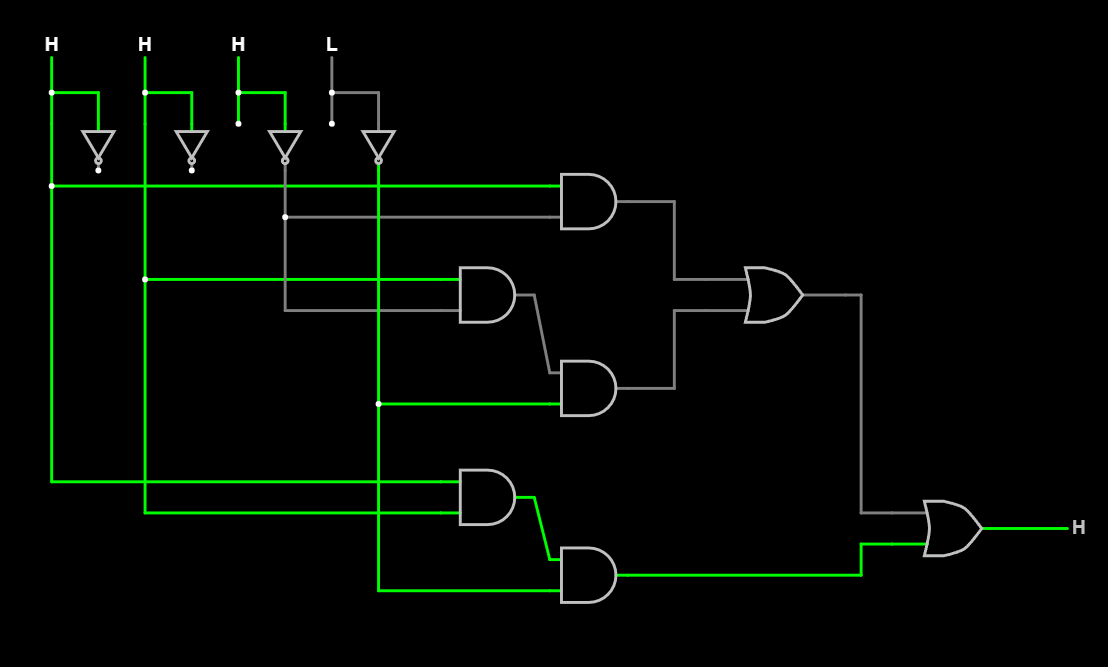
\includegraphics[width=7cm]{imagenes/2.2_S0.png}
    \caption{Circuito lógico implementado en Falstad para $S_2$}
    \label{fig:falstad_s2}
    \footnotesize\textit{Bits usados para ejemplo 1110.}
\end{figure}


\begin{figure}[h!]
    \centering
    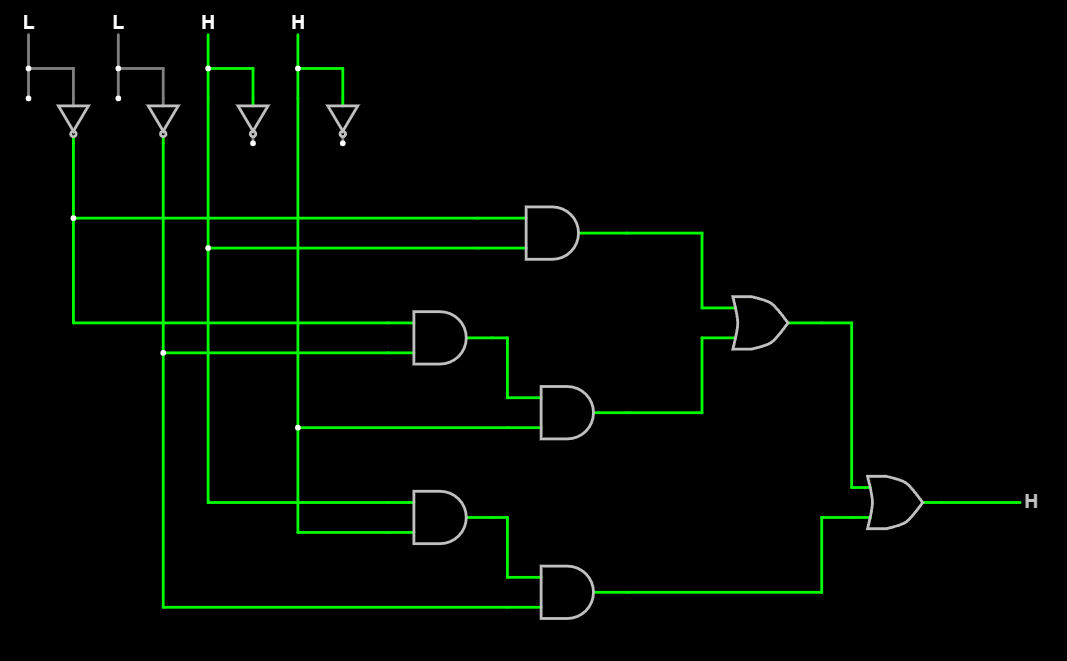
\includegraphics[width=7cm]{imagenes/2.2_S1.png}
    \caption{Circuito lógico implementado en Falstad para $S_2$}
    \label{fig:falstad_s2}
    \footnotesize\textit{Bits usados para ejemplo 0011.}
\end{figure}


\begin{figure}[h!]
    \centering
    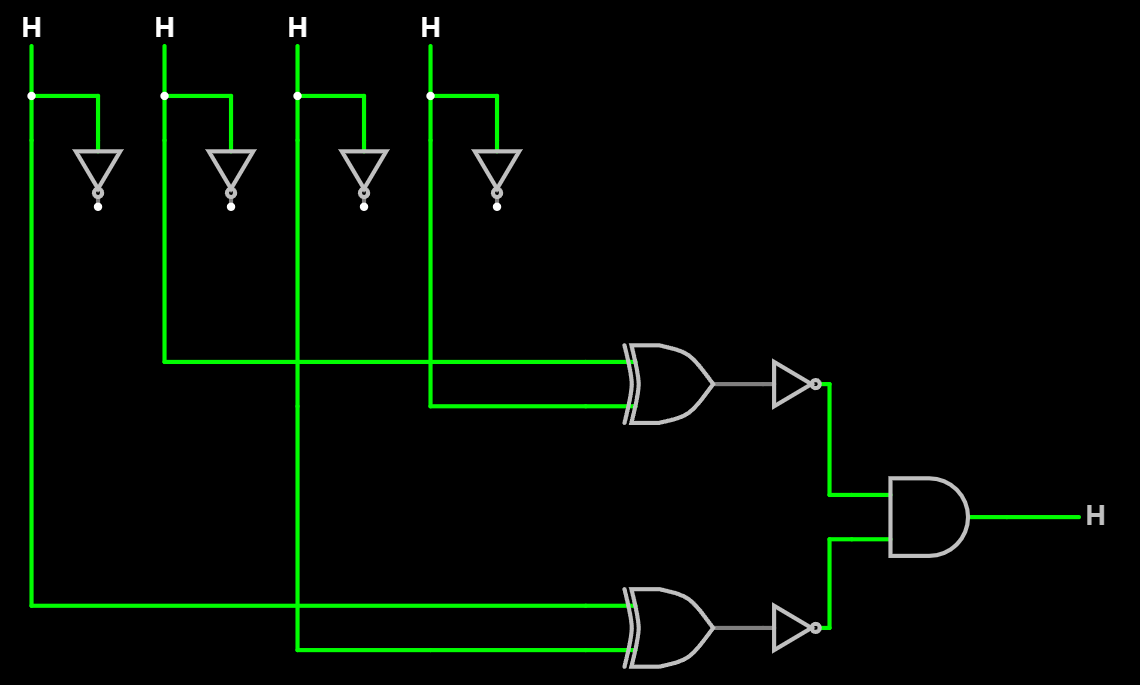
\includegraphics[width=7cm]{imagenes/2.2_S2.png}
    \caption{Circuito lógico implementado en Falstad para $S_2$}
    \label{fig:falstad_s2}
    \footnotesize\textit{Bits usados para ejemplo 1111.}
\end{figure}


\section{Imagenes de Circuitos}


\subsection{Circuito 2.1}
    Circuito lógico implementado en protoboard para la actividad 2.1
    \begin{center}
    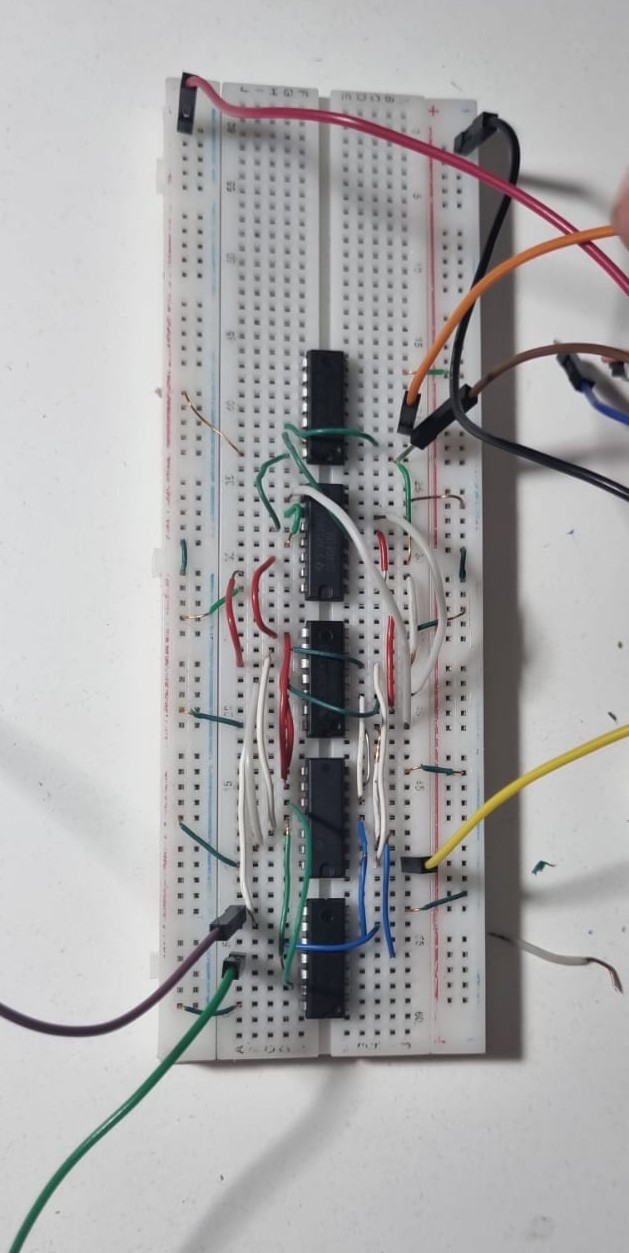
\includegraphics[width=6.3cm]{imagenes/Circuito1.jpg}
    \end{center}

\saltoPag

\subsection{Circuito 2.2}
Circuito lógico implementado en protoboard para la actividad 2.2
    \begin{center}
    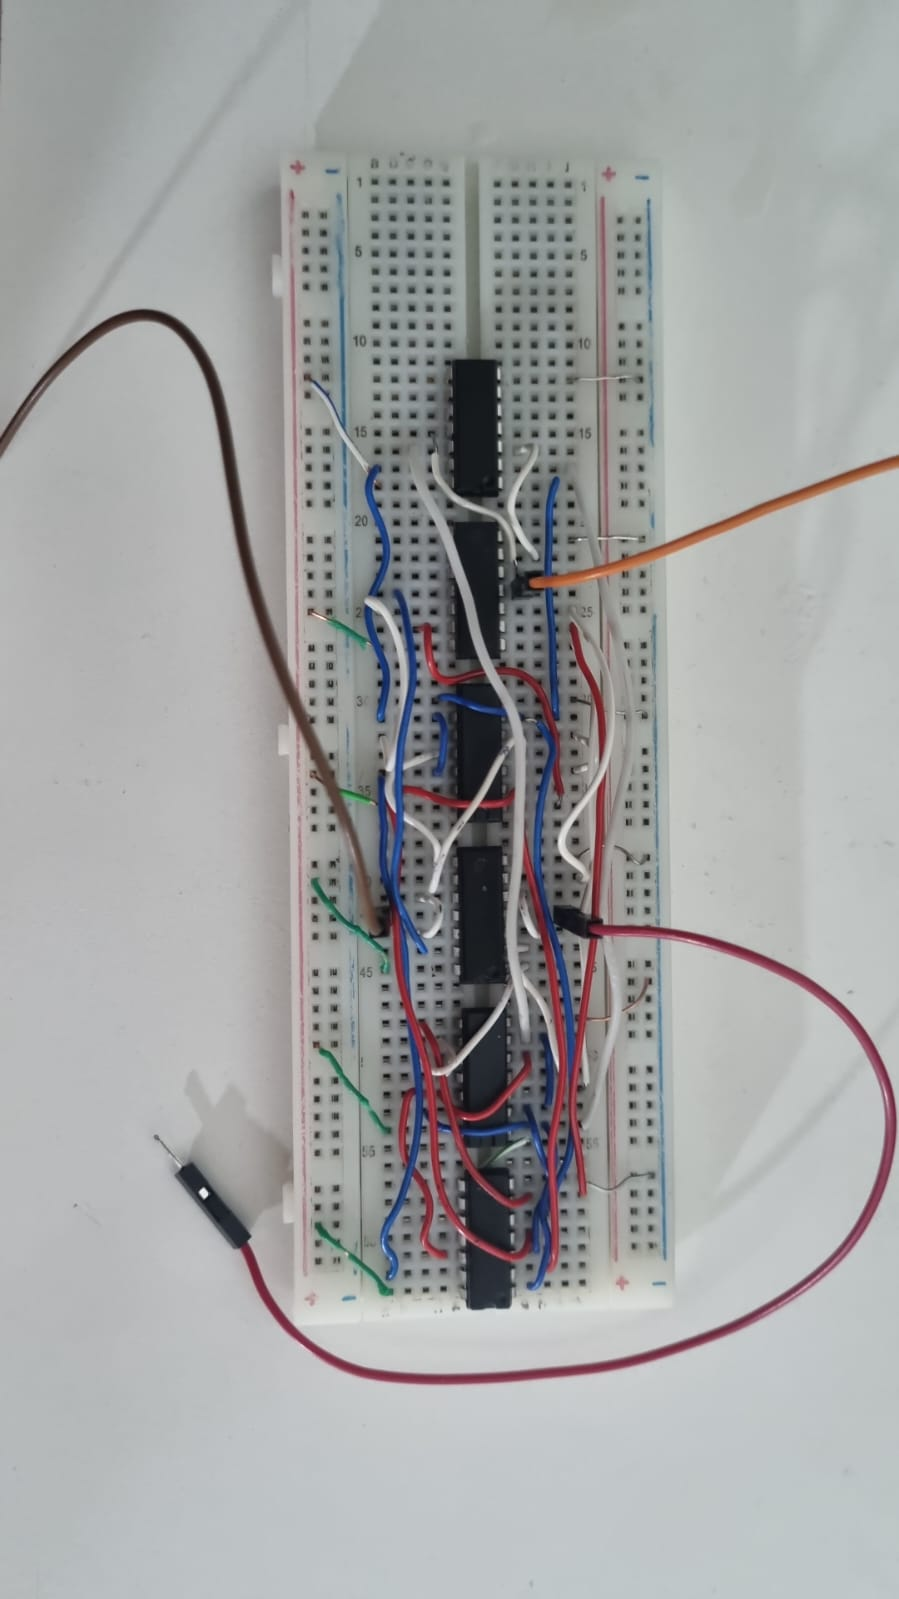
\includegraphics[width=7cm]{imagenes/Circuito2.jpg}
    \end{center}
    
